\newpage
\chapter{The elastic theory of discrete dislocations\label{elasticTheoryDislocations}}


The key aspect of the DDD method is that dislocation interactions are computed without resorting to expensive atomistic calculations. This is made possible by the 
elastic theory of dislocations, which provides semi-analytical expressions of the elastic fields (displacement, stress, strain\ldots) generated by  arbitrary dislocation loops within an infinite elastic medium. We now briefly summarize this theory,  as a special case of Mura's linearized eigendistortion theory \citep{Mura:1987wt}. 

%%%%%%%%%%%%%%%%%%%%%%%%%%%%%%%%%%%%%%%%%%%
\section{The eigendistortion problem in the infinite elastic medium\label{eigendist_classical}}
Let us consider an elastic body occupying the infinite three-dimensional space $\mathbb{R}^3$, and let $\bm u(\bm x)$ be its displacement field. We adopt here the linearized eigen-distortion framework of \cite{Mura:1987wt}, in which the main kinematic assumption  is that the displacement gradient is split additively into an elastic distortion $\bm \beta$, and an inelastic distortion $\bm \beta^\star$:
\begin{align}
u_{i,j}=\beta_{ij}+\beta^\star_{ij}\, .
\label{linear_decomposition}
\end{align}
The elastic distortion describes the local stretching of the atomic bonds and is related to stress via Hookes law ($\sigma_{ij}=\mathbb{C}_{ijkl}\beta_{kl}$). On the other hand, the inelastic distortion is the \textit{eigendistortion} of  the material, and it may contain several (additive) contributions, including plastic deformation, thermal deformation, deformation due to point defects and diffusive species in the lattice, and more. The inelastic distortion is also referred to as an \textit{eigendistortion}, because it is imagined to take place within a fictitious ``intermediate" configuration where the body is allowed to deform with incompatibilities (separations and/or interpenetrations) in order  to remain stress free. It is the subsequent elastic distortion which is responsible to develop the internal stress field necessary to remove the incompatibilities of the intermediate configuration. It will be shown that an eigendistortion field results in a state of self-stress if it is incompatible, that is if its (negative) curl 
\begin{align}
\alpha_{ij}=-\epsilon_{jkm}\beta^\star_{im,k}
\label{alpha}
\end{align}
is non vanishing. If the eigendistortion is due to dislocations, then $\bm \alpha$ can be interpreted as a tensorial density of dislocations, which  is  known as the Kr\"oner-Nye dislocation density tensor.


%In this document, we consider only the plastic contribution of the inelastic eigendistortion, so that 
%\begin{align}
%\bm\beta^\star=\bm\beta^P\, ,
%\end{align}
%where $\bm\beta^P$ is the plastic distortion caused by dislocations.

 


In the presence of a body forces density $\bm b$, 
the  static Lagrangian density of the classical linear elastic medium reads
\begin{align}
\mathcal{L}&=-\mathcal{W}-\mathcal{V}\nonumber=-\frac{1}{2}\mathbb{C}_{ijkl}\beta_{ij}\beta_{kl}+u_if_i\, ,
\end{align}
where 
\begin{align}
\label{V}
\mathcal{V}=-u_i b_i
\end{align}
is the potential of the body force density $\bm f$, while 
\begin{align}
\mathcal{W}=\frac{1}{2}\mathbb{C}_{ijkl}\eEc_{ij}\eEc_{kl}\ 
\label{W_classical}
\end{align}
is the strain energy density, which is assumed to be quadratic in the elastic strain
\begin{align}
\eEc_{ij}=\frac{1}{2}\left(\beta_{ij}+\beta_{ji}\right)
\end{align}
Here $\mathbb{C}_{ijkl}$ is the  rank-4 tensor of elastic moduli. By virtue of the symmetries
\begin{align}
\label{C}
\mathbb{C}_{ijkl}=\mathbb{C}_{jikl}=\mathbb{C}_{ijlk}=\mathbb{C}_{klij}\,,
\end{align}
it possesses up to 21 independent constants. 


The condition of static equilibrium  for displacement is expressed by the Euler-Lagrange equation
\begin{align}
\label{EL-u}
\frac{\delta \mathcal{L}}{\delta u_i}
=\frac{\partial \mathcal{L}}{\partial u_i}
-\partial_j\, \frac{\partial \mathcal{L}}{\partial (\partial_j u_i)}
%+\partial_k \partial_j\, \frac{\partial \mathcal{L}}{\partial (\partial_k \partial_j u_i)}
=-\sigma_{ij,j}-f_i
=.
\end{align}
where 
\begin{align}
\label{HL0}
\sigma_{ij}=\frac{\partial W}{\partial\eEc_{ij}}=\mathbb{C}_{ijkl}\eEc_{kl}=\mathbb{C}_{ijkl}\bEc_{kl}
\end{align}
 is the Cauchy stress tensor. Using the additive decomposition
 (\ref{linear_decomposition}), the equilibrium equation in terms of
 displacement takes the form of the following inhomogeneous Navier equation:
\begin{align}
%\mathbb{C}_{ijkl}\left(u_{k,l}-\beta^P_{kl}\right)_{,j}=
L_{ik}u_k=\mathbb{C}_{ijkl}\beta^\star_{kl,j}\,,
\label{virtualWork_classical}
\end{align}
where
\begin{align}
L_{ik}=\mathbb{C}_{ijkl}\partial_j\partial_l
\end{align} 
is the Navier differential operator. This operator admits the well-known Green's  tensor $G_{im}$ given in Eq.~(\ref{G0}). Because the Green's  tensor $G_{im}$ is the fundamental solution of the Navier operator, the particular solution of Eq.~(\ref{virtualWork_classical}) can be obtained from it by convolution with the source term. In particular, for an infinite medium the displacement field reads \cite[]{Mura:1987wt}: 
\begin{align}
u_{i}&= - \mathbb{C}_{mnpq}G_{im}*\beta^\star_{pq,n} \nonumber\\
&=- \mathbb{C}_{mnpq}G_{im,n}*\beta^\star_{pq}  && \text{(generalized Volterra equation)}\,.
\label{eigen_displ} 
\end{align}
In Eq.~(\ref{eigen_displ}) we have introduced the symbol $*$ to indicate convolution over the infinite three-dimensional space. 
With dislocation theory in mind, Eq.~(\ref{eigen_displ}) can be considered a \textit{generalized Volterra solution} valid for an arbitrary source of eigendistortion. 

An expression for the displacement gradient split into elastic and plastic contributions is obtained  using the Mura-Willis procedure: 
\begin{align}
u_{i,j}&=-\mathbb{C}_{mnpq}G_{im,n}*\bPc_{pq,j}
=-\mathbb{C}_{mnpq}G_{im,n}*\left(\bPc_{pj,q}+\epsilon_{qjr}\alpha_{pr}\right)\nonumber\\
&=-\mathbb{C}_{mnpq}G_{im,nq}*\bPc_{pj}-\mathbb{C}_{mnpq}\epsilon_{qjr}G_{im,n}*\alpha_{pr}\nonumber\\
&=-L_{pm}G_{im}*\bPc_{pj}-\mathbb{C}_{mnpq}\epsilon_{qjr}G_{im,n}*\alpha_{pr}=\delta_{ip}\delta*\bPc_{pj}-\mathbb{C}_{mnpq}\epsilon_{qjr}G_{im,n}*\alpha_{pr}\nonumber\\
&=\bPc_{ij}+\mathbb{C}_{mnpq}\epsilon_{jqr}G_{im,n}*\alpha_{pr}
\label{disp_grad_class}
\end{align}
From \eqref{disp_grad_class}, the elastic distortion follows immediately as
\begin{align}
\bEc_{ij}=\mathbb{C}_{mnpq}\epsilon_{jqr}G_{im,n}*\alpha_{pr}\,. && \text{(Mura-Willis equation)}
\label{betaE_class}
\end{align}
Clearly, the Cauchy stress field $\sigma_{ij}$ can be obtained from \eqref{betaE_class} using the Hooke's law~(\ref{HL0}). 
\begin{align}
\sigma_{ij}=\mathbb{C}_{ijkl}\mathbb{C}_{mnpq}\epsilon_{lqr}G_{km,n}*\alpha_{pr} &&
\text{(anisotropic Peach-Koehler stress equation)}\,.
\label{PK0}
\end{align}
Note that elastic distortion \eqref{betaE_class} and stress \eqref{PK0} depend on the eigendistortion $\bm \beta^\star$ only through its curl $\bm \alpha$, and therefore they vanish is  $\bm \beta^\star$ is compatible.

We are now interested in obtaining an alternative expression of the displacement field \eqref{eigen_displ} where the contribution of elastic and plastic distortions appear in separate additive terms. Following  \citep{Lazar:2013jb},  we first take the derivative of Eq.~(\ref{linear_decomposition}) with respect to $x_j$ in order to obtain the Poisson equation:
\begin{align}
\Delta u_i=u_{i,jj}=\beta_{ij,j}+\beta^\star_{ij,j}\ ,
\label{linear_decomposition_div}
\end{align}
where $\Delta=\partial_j\partial_j$ is the Laplace operator. Second we ``invert" Eq. (\ref{linear_decomposition_div}) using the Green's  function\footnote{The three-dimensional Green's  function of the  Laplace operator is~\citep{Wl}
\begin{align}
\GP(\bm R)=-\frac{1}{4\pi R}
\label{Green_Poiss}
\end{align}
where $R=\sqrt{\bm R\cdot\bm R}$ is the Euclidean norm of $\bm R$.
} of the Laplace operator $\GP$: 
\begin{align}
u_{i}=\left(\beta^\star_{ij,j}+\beta_{ij,j}\right)*\GP = \beta^\star_{ij}*\GP_{,j}+\beta_{ij,j}*\GP\, .
\label{disp_green}
\end{align}
It will be clearer in the following sections that Eq.~(\ref{disp_green}) can be considered as a \textit{generalized Burgers equation}. In fact, although Eq.~(\ref{disp_green}) is valid for an arbitrary source of  eigendistortion in an anisotropic medium, its name is well-justified in the case of dislocation loops because the term $ \beta^\star_{ij}*\GP_{,j}$ corresponds to the contribution of the solid angle subtended by a loop, which was first isolated by Burgers \citep{Burgers:1939ui,Burgers:1939vn} in the classical isotropic case. Substituting Eq.~(\ref{betaE_class}) in (\ref{disp_green}), we find the
generalized Burgers solution for the displacement field (see also \citet{Lazar:2013jb}):
\begin{align}
u_i
&=\GP_{,j}*\beta^\star_{ij}-\mathbb{C}_{mnpq}\epsilon_{jqr}F_{jnim}*\alpha_{pr}  && \text{(generalized Burgers equation)}\,.
\label{gen_Burg0}
\end{align}
Note that, following \citet{Kirchner:1983} and \citet{Lazar:2013jb}, in Eq.~(\ref{gen_Burg0}) we have introduced the fourth-rank tensor $F_{jnim}$ defined as:
\begin{align}
F_{jnim}=-G_{im,jn}*\GP \,.
\label{F_classical}
\end{align}
Similar to the Green's  tensor, also the ``$\bm F$-tensor" has an explicit form, which is given in Eq.~(\ref{F0}). 
%

The $\bm F$-tensor is also useful in deriving a compact expression for the
interaction energy between two sources of eigendistortion. 
In fact, the elastic interaction energy between two sources of eigendistortion, labeled A and B respectively, can be obtained as\footnote{
In order to prove \eqref{wAB_classical}, we
use the following representation of the gradient of the Green's  tensor in terms
of the $\bm F$-tensor:
   \begin{align}
G_{im,j}=G_{im,jnn}*\GP=-F_{jnim,n}\,.
\end{align}
With this, a derivation of \eqref{wAB_classical} goes as follows: 
 \begin{align} 
 W_{AB}&
= \int_{\mathbb{R}^3}\sigma^{(A)}_{il}\, \beta^{(B)}_{il}\dV%\nonumber\\
= \int_{\mathbb{R}^3}\mathbb{C}_{ilmn}\epsilon_{npq}\mathbb{C}_{rstp}\left(G_{mr,s}*\alpha^{(A)}_{tq}\right)\, \beta^{(B)}_{il}\dV
=- \int_{\mathbb{R}^3}\mathbb{C}_{ilmn}\epsilon_{npq}\mathbb{C}_{rstp}\left(F_{skmr,k}*\alpha^{(A)}_{tq}\right)\, \beta^{(B)}_{il}\dV\nonumber\\
&= \int_{\mathbb{R}^3}\mathbb{C}_{ilmn}\epsilon_{npq}\mathbb{C}_{rstp}\left(F_{skmr}*\alpha^{(A)}_{tq}\right)\, \beta^{(B)}_{il,k}\dV
= \int_{\mathbb{R}^3}\mathbb{C}_{ilmn}\epsilon_{npq}\mathbb{C}_{rstp}\left(F_{skmr}*\alpha^{(A)}_{tq}\right)\, \left(\beta^{(B)}_{ik,l}+\epsilon_{jkl}\alpha^{(B)}_{ij}\right) \dV\nonumber\\
&= -\int_{\mathbb{R}^3}\underbrace{\mathbb{C}_{ilmn}\epsilon_{npq}\mathbb{C}_{rstp}\left(G_{mr,skl}*\alpha^{(A)}_{tq}\right)}_{\sigma_{il,lk}}*\GP\, \beta^{(B)}_{ik} \dV+
 \int_{\mathbb{R}^3}\epsilon_{jkl}\mathbb{C}_{ilmn}\epsilon_{npq}\mathbb{C}_{rstp}\left(F_{skmr}*\alpha^{(A)}_{tq}\right)\, \alpha^{(B)}_{ij} \dV\nonumber\\
 &=\int_{\mathbb{R}^3}\epsilon_{jkl}\mathbb{C}_{ilmn}\epsilon_{npq}\mathbb{C}_{rstp}\left(F_{skmr}*\alpha^{(A)}_{tq}\right)\, \alpha^{(B)}_{ij} \dV \nonumber\,.
 \end{align}
This result shows that the interaction energy between two sources of eigendistortion depends only on their curls. Therefore it can be regarded as an anisotropic generalization of Blin's equation \citep{Blin:1955wh}, valid for arbitrary sources of eigendistortion. Surprisingly, such fundamental result has long been missing in anisotropic eigendistortion theory, and it was   found only recently by \cite{Lazar:2013jb} using the method of stress functions. 
To our knowledge, the derivation above is the first without stress functions.
}:
 \begin{align} 
 W_{AB}
 &=\int_{\mathbb{R}^3}\epsilon_{jkl}\mathbb{C}_{ilmn}\epsilon_{npq}\mathbb{C}_{rstp}\left(F_{skmr}*\alpha^{(A)}_{tq}\right)\, \alpha^{(B)}_{ij} \dV && (\text{generalized Blin's interaction energy equation})\,.
 \label{wAB_classical}
 \end{align}




while  the configurational force exerted on
the eigendistortion can be computed from the  divergence of  Eshelby's stress
tensor. This  gives the 
Peach-Koehler force on the eigendistortion:
%Clearly, in order to obtain the Peach�Koehler force between two dislocation loops it is sufficient to substitute the Peach� Koehler stress equation (7b) into (12).
%The configurational force exerted on the eigendistortion can be computed form the  divergence of the Eshelby stress tensor: 
\begin{align}
\mathcal{F}_k=\int_{\mathbb{R}^3}\left(W\delta_{kj}-\sigma_{ij}\bEc_{ik}\right)_{,j}\dV=\int_{\mathbb{R}^3}\epsilon_{kjm}\sigma_{ij}\alpha_{im}\dV\,.
\label{EshelbyStress_classical}
\end{align}

%%%%%%%%%%%%%%%%%%%%%
\subsection{Isotropic media}


 
%%%%%%%%%%%%%%%%%%%%%%%%%%%%%%%%%%%%%%%%%%%
\section{Dislocation loops\label{disloC_classical}}
 
 \begin{figure}[t]
\centering
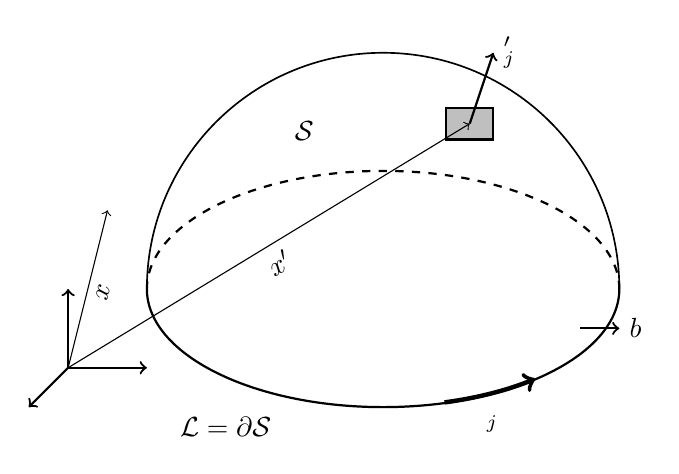
\begin{tikzpicture}
  \draw[semithick] (0,0) arc (0:180:3);
  \draw (-4,2) node {$\mathcal{S}$};
  \draw[dashed, thick] (0,0) arc [x radius=3, y radius=1.5, start angle=0, end angle=180];
  \draw[thick] (-6,0) arc [x radius=3, y radius=1.5, start angle=180, end angle=360];
  \draw[ultra thick, ->] (-2.22,-1.44) arc [x radius=3, y radius=1.5, start angle=285, end angle=310]
    node[below left, outer sep=10pt] {$\dL_j$};
  \filldraw[fill=gray!50!white, thick] (-2.2,2.3) rectangle (-1.6,1.9);
  \draw[thick, ->] (-1.9,2.1) -- (-1.6,3) node[right] {$\dA_j'$};
  \draw (-5,-1.5) node[below] {$\mathcal{L}=\partial\mathcal{S}$};
  \draw[->,thick] (-7,-1) -- (-7,-0); 
\draw[->,thick] (-7,-1) -- (-6,-1); 
\draw[->,thick] (-7,-1) -- (-7.5,-1.5); 
\draw[->] (-7,-1) --(-1.9,2.1)  node [sloped,below,text centered,midway]{$ \bm x'$}; 
\draw[->] (-7,-1) --(-6.5,1)  node [sloped,below,text centered,midway]{$ \bm x$}; 
\draw[->,thick] (-0.5,-0.5) --(-0,-0.5)  node [sloped,right,text centered]{$ \bm b$}; 
\end{tikzpicture}
\caption{The plastic distortion is concentrated on the surface $\mathcal{S}$, which is bounded by the dislocation line $\mathcal{L}=\partial\mathcal{S}$.}
\label{fig:dislocation_loop} 
\end{figure}
Let us know assume that the eigendistortion $\bm \beta^\star$ is only due to plastic deformation cause by dislocations, that is
\begin{align}
\bm \beta^\star=\bm \beta^P
\end{align}
The key equations of classical dislocation theory are now obtained by prescribing  the form of the eigendistortion tensor $\bm \beta^P$. For a dislocation extending over a surface $\mathcal{S}$,  the classical plastic eigendistortion tensor is taken in following form:
\begin{align}
\bPc_{kl}(\bm x)=-\int_\mathcal{S}\delta(\bm x-\bm x')b_k\dA_l'\, ,
\label{dislocation_distortion_classical}
\end{align}
where $\delta$ is the Dirac delta function, and $b_i$ is the displacement jump across $\mathcal{S}$, or Burgers vector. For a Volterra dislocation, as opposed to a Somigliana dislocation,  the Burgers vector is constant. In this case,  the  tensor $\alpha_{ij}=-\epsilon_{jkm}\bPc_{im,k}$ turns out to be concentrated on the dislocation line, that is the closed line $\mathcal{L}=\partial\mathcal{S}$ bounding the surface $\mathcal{S}$, and it is known as the \textit{dislocation density tensor}:
\begin{align}
\alpha_{ij}(\bm x)=\oint_{\mathcal{L}}\delta(\bm x-\bm x')b_i\dL_j'\, .
\label{dislocation_alpha_classical}
\end{align}
The rate of plastic distortion can be written in terms of the local dislocation velocity $w_k$ as
\begin{align}
\dot{\beta}^P_{ij}(\bm x)
=-\oint_{\mathcal{L}}\delta(\bm x-\bm x')b_i\epsilon_{jkm}w_k(\bm x')\dL_m'\,.
\label{plasticDistortionRateLoop}
\end{align}

Using the special forms (\ref{dislocation_distortion_classical}) and (\ref{dislocation_alpha_classical}) in the results obtained in the previous section we find all the key equations of classical dislocation theory in the anisotropic case. Letting $\bm R=\bm x-\bm x'$, these are:
\begin{subequations}
\begin{align}
u_i(\bm x)
&=-\frac{b_i\, \Omega(\bm
  x)}{4\pi}-\oint_{\mathcal{L}}\mathbb{C}_{mnpq}\epsilon_{jqr}b_pF_{jnim}(\bm
R)\dL_r' && \text{(anisotropic Burgers equation)}\\
\bEc_{ij}(\bm x)&=\oint_{\mathcal{L}}\mathbb{C}_{mnpq}\epsilon_{jqr}G_{im,n}(\bm R)b_p\dL_r' && \text{(Mura-Willis equation)}\\
\sigma_{ij}(\bm
x)&=\oint_{\mathcal{L}}\mathbb{C}_{ijkl}\mathbb{C}_{mnpq}\epsilon_{lqr}G_{km,n}(\bm
R)b_p\dL_r' && \text{(anisotropic Peach-Koehler stress equation)}\label{classicaCauchyStress}\\
W_{AB}&=\oint_{\mathcal{L}_A}\oint_{\mathcal{L}_B}\epsilon_{jkl}\mathbb{C}_{ilmn}\epsilon_{npq}\mathbb{C}_{rstp}F_{skmr}(\bm R)\, b^{A}_{t} b^{B}_{i} \dL^A_{q}\dL^B_{j}&&\text{(anisotropic Blin's formula) }\\
\mathcal{F}_k&=\oint_\mathcal{L}\epsilon_{kjm}\sigma_{ij}b_i\dL_m&&\text{(Peach-Koehler force)}
\end{align}
\label{class_aniso_all}
\end{subequations}
Note that, in the Burgers equation, we have introduced the solid angle  $\Omega(\bm x)$ subtended by the loop from the relationship  $\GP_{,j}*\bPc_{ij}=-{b_i\, \Omega}/{4\pi}$, which yields:
\begin{align}
\Omega(\bm x)=4\pi\int_\mathcal{S}\GP_{,j}\dA_j'=\int_\mathcal{S}\frac{R_j}{R^3}\dA_j'\, .
\end{align}

The kernel of Eq.~\eqref{}








%%%%%%%%%%%%%%%%%%%%%%%%%%%%%%%%%%%%%%%%%%
\section{The eigendistortion problem in the finite elastic medium: the superposition principle}

So far we have discussed the DDD method in the infinite elastic medium. However, many applications in micro-plasticity, such as micro indentation and micro-pillar compression, require that the dislocation network be embedded in a finite domain subject to prescribed boundary conditions. In order to extend the DDD method to finite domains, let us consider the eigenstrain problem in a finite domain   $\mathcal{B}$. In this case, the displacement field $u_k$ must satisfy the following boundary value problem (BVP) :
\begin{align}
\begin{cases}
\sigma_{ij}=c_{ijkl}\left(u_{k,l}-\beta^\star_{kl}\right) & \mbox{in }\mathcal{B}\\
\sigma_{ij,j}=0 & \mbox{in }\mathcal{B}\\
\sigma_{ij}\hat{n}_j=p_i & \mbox{on } \partial_N\mathcal{B}\\
u_i=\overline{u}_i & \mbox{on } \partial_D\mathcal{B}
\end{cases}
\label{BVPfinite}
\end{align}
where $p_i$ is the prescribed traction on the portion of the boundary $\partial_N\mathcal{B}$, and $\overline{u}_i$ is the prescribed displacement on the portion of the boundary $\partial_D\mathcal{B}$. Ideally, the BVP~(\ref{BVPfinite}) could be solved at each DDD step by incrementally updating $\beta^P_{ij}$ using its rate from eq.~(\ref{plasticDistortionRateLoop}). In a finite element framework this would provide the nodal displacements, from which the total stress could be computed and used to drive the discrete dislocation system inside $\mathcal{B}$. Practically, however, this approach is unfeasible because stresses, obtained as derivatives of displacement shape functions, would result in smooth fields which fail to  capture  sharp gradients in proximity of dislocation lines. In order to overcome this issue, an alternative formulation has been sought (c.f. \cite{eshelby1979boundary,Lubarda:1993uc,vanderGiessen:1995tm,Deng:2008fs,Weygand:2002tq}),  where the problem is decomposed into two auxiliary problems. The first problem, with infinite domain $\mathbb{R}^3$, consists in finding $u_i^\infty$ such that:
\begin{align}
\begin{cases}
\sigma^{\infty}_{ij}=c_{ijkl}(u^{\infty}_{k,l}-\beta^{P}_{kl}) & \mbox{in }\mathbb{R}^3\\
\sigma^{\infty}_{ij,j}=0 & \mbox{in }\mathbb{R}^3
\end{cases}
\label{BVPinfinite}
\end{align}
The second is a purely elastic ``correction" problem, with domain $\mathcal{B}$ consisting in finding $u_i^c$ such that:
\begin{align}
\begin{cases}
\sigma^c_{ij}=c_{ijkl}u^c_{k,l}& \mbox{in }\mathcal{B}\\
\sigma^c_{ij,j}=0 & \mbox{in }\mathcal{B}\\
\sigma^c_{ij}\hat{n}_j=p_i- \sigma^\infty_{ij}\hat{n}_j& \mbox{on } \partial_N\mathcal{B}\\
u_i^c=\overline{u}_i-u^\infty_i & \mbox{on } \partial_D\mathcal{B}
\end{cases}
\label{BVPcorrection}
\end{align}
The rationale behind this decomposition is clearly that (\ref{BVPinfinite}) is the standard dislocation eigenstrain problem in an infinite medium that we already solved in the previous sections. The total solution is clearly obtained as a sum: $u_i=u_i^\infty+u_i^c$ and the total stress field $\sigma_{ij}=\sigma_{ij}^\infty+\sigma_{ij}^c$ is used to drive dislocations in the finite-domain version of DDD.

%\begin{figure}[t]
%\centering\begin{tikzpicture}
%\draw [very thick] (-4,0) rectangle (4,3);
%\fill [fill=red!20!white] (-1.5,3.03) rectangle (1.5,5);
%\node at (0,4) {$\bm\beta^{P*}$};
%\node at (-3.5,0.5) {$\mathcal{B}$};
%  \begin{scope}[thick,decoration={
%    markings,
%    mark=at position 0.5 with {\arrow{>}}}
%    ] 
%    \draw[red!50!white,postaction={decorate}] (-1.5,5)--(1.5,5);
%    \draw[red!50!white,postaction={decorate}] (-1.5,3.03)--(-1.5,5);
%    \draw[red!50!white,postaction={decorate}] (1.5,5)--(1.5,3.03);
%    \draw[red!50!white,postaction={decorate}] (1.5,3.03)--(-1.5,3.03);
%\end{scope}
%\node at (0,5.2) {$\infty$};

% \begin{scope}[shift={(1.5,1)}]
%    \draw [blue,thick,domain=0:7.8540,variable=\t,smooth,samples=150]
%        plot ({\t r}: {0.032*\t*\t});
%  \end{scope}
%   \begin{scope}[shift={(-1.5,1)}]
%    \draw [blue,thick,domain=0:7.8540,variable=\t,smooth,samples=150]
%        plot ({-\t r}: {-0.032*\t*\t});
%  \end{scope}
  
%  \begin{scope}[thick,decoration={
%    markings,
%    mark=at position 0.5 with {\arrow{>}}}
%    ] 
%    \draw[blue,postaction={decorate}] (-1.5,2.97)--(1.5,2.97);
%\end{scope}
%\draw[->,thick] (2.5,1) --(3,0.5)  node [sloped,right,text centered]{\textcolor{black}{$ \bm b$}}; 
%\draw[->,thick] (1.25,4) --(1.75,3.5)  node [sloped,right,text centered]{\textcolor{black}{$ \bm b$}}; 
%\end{tikzpicture}
%\caption{Construction used for the solution of the BVP (\ref{BVPcorrection}). For each dislocation segment on the domain boundary a loop with the same Burgers vector and opposite line direction is constructed outside the integration domain, and encloses the virtual slip surface $\beta^{P*}$. One portion of the external loop coincides with the boundary segment, and the opposite side is pushed to infinity in the direction of the boundary normal.}
%\label{BVPStrategy}
%\end{figure}

From a numerical viewpoint, it is interesting to ask; what is the distribution of $\beta^P_{ij}$ outside $\mathcal{B}$ in (\ref{BVPinfinite})? We shall call this quantity $\beta^{P*}_{ij}$. In fact, although the solution to the problems (\ref{BVPinfinite}) and (\ref{BVPcorrection}) depend individually on $\beta^{P*}_{ij}$, it is easy to see that the total solution is independent of  $\beta^{P*}_{ij}$. Therefore $\beta^{P*}_{ij}$ can be chosen arbitrarily\footnote{We observe that the arbitrariness of $\beta^{P*}_{ij}$ implies that also its bounding curve (or virtual dislocation line) is arbitrary, in agreement with the ``mirror image construction" of \cite{Weygand:2002tq}  and the ``independence of the total stress on the choice of virtual segments'' mentioned in \cite{Weinberger:2009fk}.}.  The arbitrariness of $\beta^{P*}_{ij}$ can be exploited in the numerical implementation. To see how, we can cast  (\ref{BVPcorrection}) in its   corresponding Galerkin weak form
\begin{align}
\int_\mathcal{B}c_{ijkl}u^c_{k,l}\tilde{u}_{i,j}d\mathcal{V}=\int_{\partial_N\mathcal{B}}\left(p_i- \sigma^\infty_{ij}\hat{n}_j\right)\tilde{u}_id\mathcal{A}
\label{BVPcorrectionWeak}
\end{align} 
and notice that the RHS involves a surface integral  of the stress field  $\sigma^\infty_{ij}$ induced by the dislocation network. When a dislocation segment reaches the domain boundary, the numerical evaluation of this integral becomes challenging. This numerical difficulty can be  overcome using the construction shown in Fig.~\ref{BVPStrategy}. In fact, because $\beta^{P*}_{ij}$ is arbitrary, it is possible to add an external loop with the same Burgers vector of the boundary segment and opposite line direction, constructed so that one side of the loop overlaps with the boundary segment, and the opposite side is pushed to infinity along the direction of the boundary normal vector. In this way, because the contributions of the overlapping segments cancel out, the line integral involved in the calculation of $\sigma^{\infty}_{ij}$ can be limited to the portion of the dislocation configuration strictly inside the domain, and the virtual straight dislocation lines extending from the domain boundary to infinity. Notice that this construction unambiguously defines $\beta^{P*}_{ij}$ and the surface over which it extends, a fundamental requirement for the calculation of $u^\infty_i$ needed to satisfy displacement boundary conditions in the BVP (\ref{BVPcorrection}). 
